
\begin{figure}[h]
    \centering  
    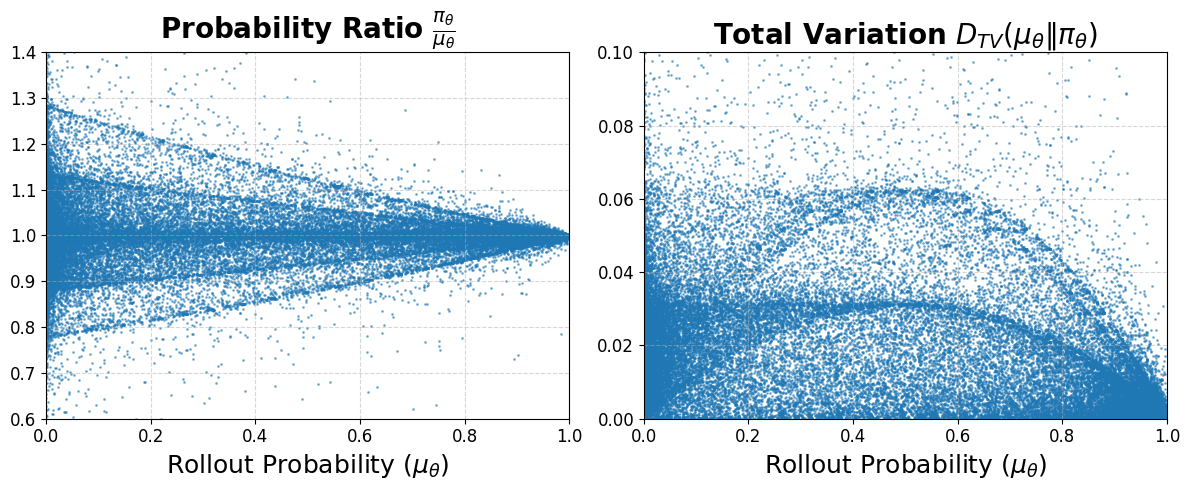
\includegraphics[width=\linewidth]{figs/moe_prob_ratio_tv_1.png}
    \caption{The plots show numerical differences between training and inference engines for Qwen3-30B-A3B-Base with identical parameters. \textbf{(Left)} The token-level probability ratio (used in PPO) is highly volatile for low-probability tokens. \textbf{(Right)} The token-level TV divergence (used in DPPO) is more stable.
    %  $D_{\mathrm{TV}}(\rolloutpi(\cdot|s_t)\|\trainerpi(\cdot|s_t))$
    This highlights a key flaw of PPO's clipping: it over-penalizes low-probability tokens, which can slow down learning; and under-penalizes high-probability tokens, which can permit large, destabilizing updates.
    }  
    % \vspace{-0.4cm}
\label{fig:moe_prob_ratio_tv}  
\end{figure}

% \vspace{-0.5cm}
\section{Introduction}  
\label{sec:introduction}  


Reinforcement learning (RL) is a foundational paradigm for fine-tuning Large Language Models (LLMs), enabling alignment with human preferences \citep{ouyang2022training, rafailov2023direct} and complex reasoning tasks \citep{guo2025deepseekr1, qi2025optimizing}.
In practice, LLM RL is often off-policy: an inference engine samples rollouts, while a trainer engine computes gradients. Even when the two engines use the same model parameters, \emph{training-inference mismatch}~\citep{yao2025offpolicy, qi2025defeating, zheng2025stabilizing} can make their token distributions differ. Practical systems also use collected rollouts for several minibatch updates to improve throughput~\citep{liu2025deepseek}. These choices make it essential to control how far each update moves the trained policy from the policy that generated the data. \looseness=-1

Proximal Policy Optimization (PPO\footnote{We denote PPO by its ratio-clipping loss, regardless of advantage estimation. Under this definition, GRPO is a PPO variant.}) \citep{schulman2017proximal} is the dominant algorithm in this setting because it is simple and scalable. Its main safeguard is ratio clipping. If the probability ratio between the new policy and the behavior policy becomes too large or too small on a sampled token, PPO clips the objective. This rule is meant to keep updates inside a \emph{trust region}, where monotonic improvement is theoretically guaranteed \citep{schulman2015trust}.

Despite its widespread adoption, we argue that PPO’s core mechanism, ratio clipping, is structurally ill-suited for the expansive, long-tailed vocabularies inherent to LLMs. Although motivated by Trust Region Policy Optimization (TRPO) \citep{schulman2015trust}, which constrains KL or Total Variation (TV) divergence of policy distributions, PPO instead clips the probability ratio of the sampled token. This ratio is only a noisy, single-sample estimate of the true policy divergence. While this approximation may suffice for classical RL environments with limited action spaces, it fails in the LLM regime because the ratio depends strongly on the original token probability. For example, increasing a rare token's probability from $10^{-5}$ to $10^{-3}$ gives a ratio of $100$ and triggers clipping, although the moved probability mass is small. Conversely, decreasing a high-probability token from $0.99$ to $0.8$ moves much more mass, yet the ratio may remain inside a typical clipping range.

Training-inference mismatch makes this problem worse. As illustrated in \Cref{fig:moe_prob_ratio_tv}, the probability ratio becomes highly volatile for low-probability tokens, while TV divergence remains stable. Consequently, PPO creates a sub-optimal learning dynamic: updates to low-probability tokens are aggressively over-penalized, slowing learning, while updates to high-probability tokens are under-penalized, risking instability. This implicit bias necessitates a fundamental rethinking of the trust region approach in LLM fine-tuning to ensure both efficiency and stability.

To address this limitation, we propose Divergence Proximal Policy Optimization (DPPO), which replaces ratio-based clipping with a constraint based on policy divergence. Rather than relying on noisy single-sample ratios, DPPO directly estimates policy divergence (e.g., TV or KL divergence). To ensure memory feasibility, we introduce two efficient approximations, Binary and Top-K divergence, which capture essential distributional shifts with negligible overhead. This allows DPPO to rigorously distinguish between safe and unsafe updates, effectively resolving the problems of over- and under-constraining inherent in standard PPO.


In this work, we provide a comprehensive rethinking of the trust region in the context of LLM fine-tuning. Our contributions are threefold. \textbf{Theoretical Formulation}: We derive policy improvement bounds specifically tailored to the finite-horizon, undiscounted setting of LLM generation, establishing a rigorous theoretical foundation for trust-region methods in this domain. \textbf{Stability and Efficiency Analysis}: We isolate the primary sources of training instability to provide practical stabilization guidelines, while further highlighting the significant role that low-probability tokens play in driving exploration. \textbf{Algorithmic Performance}: We demonstrate that DPPO achieves superior stability and final performance compared to existing methods like GRPO, providing a robust new framework for RL-based fine-tuning.

